\documentclass[border=10pt]{standalone}
\usepackage{tikz}\usepackage{amsmath}\usetikzlibrary{arrows.meta,decorations.markings}
\begin{document}
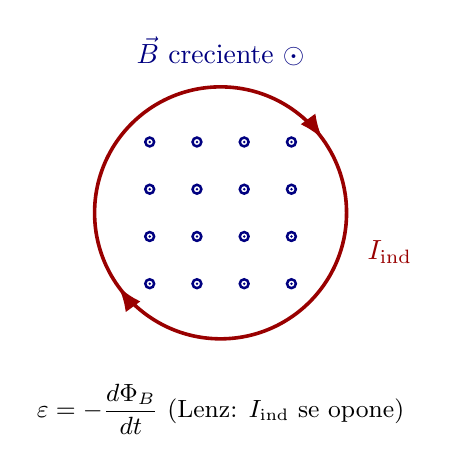
\begin{tikzpicture}[line width=0.9pt,>={Latex[length=2.4mm]}]
  % B saliente creciente
  \foreach \x in {-0.9,-0.3,0.3,0.9} \foreach \y in {-0.9,-0.3,0.3,0.9}{
     \draw[blue!50!black] (\x,\y) circle(1.6pt); \fill[blue!50!black] (\x,\y) circle(0.5pt);}
  \node[blue!50!black] at (0,2.05){$\vec B$ creciente $\odot$};
  % espira con corriente inducida (horario, se opone) -- arco horario
  \draw[line width=1.3pt,red!60!black,decoration={markings,
        mark=at position 0.15 with {\arrow{Latex}},
        mark=at position 0.65 with {\arrow{Latex}}},postaction={decorate}]
        (0,0) ++(90:1.6) arc (90:-270:1.6);
  \node[red!60!black] at (2.15,-0.5){$I_{\text{ind}}$};
  \node at (0,-2.5){\small $\displaystyle \varepsilon=-\frac{d\Phi_B}{dt}$ (Lenz: $I_{\text{ind}}$ se opone)};
\end{tikzpicture}
\end{document}
